%=======================+=========================
%==============   The beamline     ===============
%=================================================

\section[The beam line and coherent photon source (Stuart)]{The beam line and coherent photon source \label{sec:beamline}}

%\begin{figure}[t]
%\begin{center}
%   %\includegraphics[viewport=1 1 790 %540,clip,angle=0,width=0.98\linewidth]{figs/mainmachine_beamline_dwg}
%\end{center}
%\caption{Schematics of the accelerator and the beam extraction system.
%        }
%\label{fig:beam:cebaf-dwg} 
%\end{figure}


The Hall D complex has been described in Section \ref{sec:gluexexperiment:complex} and is shown schematically in Fig.~\ref{fig:beam:Draw_beamline}, which shows the Tagger Hall, the collimator cave and Hall D itself. The photon beam is produced in the Tagger Hall, which is described in more detail in Section\,\ref{sec:tag}.
The dimensions are measured in centimeters unless specified differently.

\begin{figure}[t]
\begin{center}
%   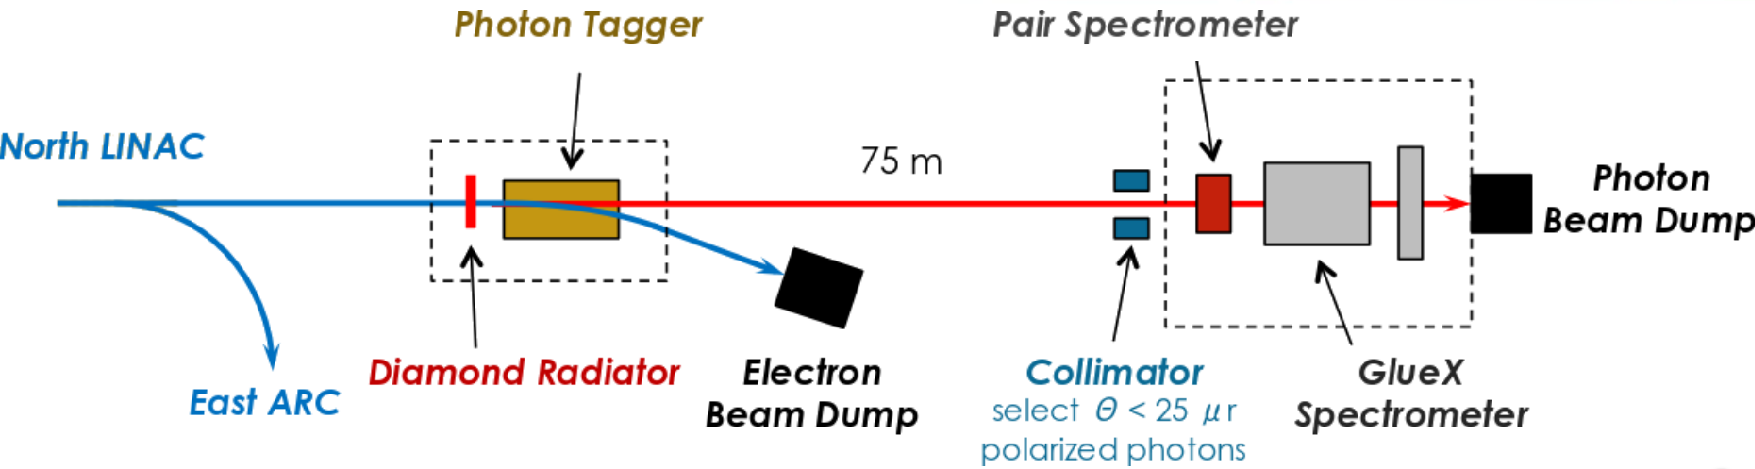
\includegraphics[clip=true,width=0.98\linewidth]{figures/gx_beamline_0}
 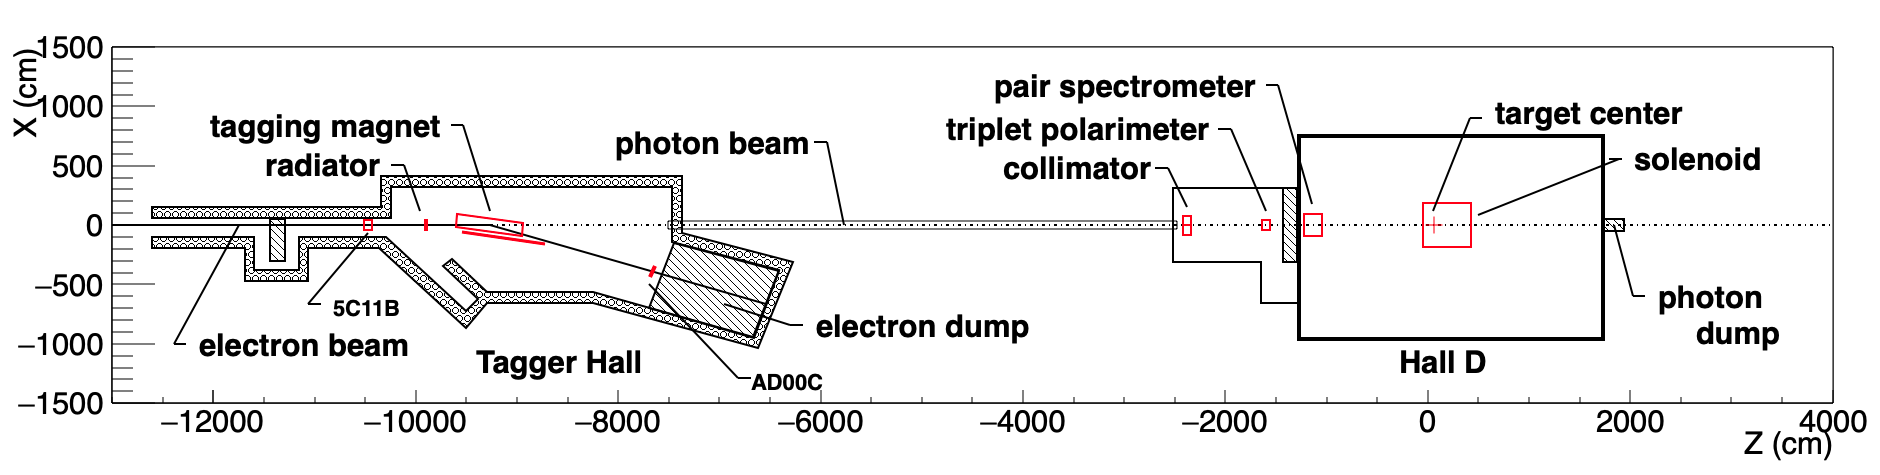
\includegraphics[clip=true,width=0.98\linewidth]{figures/Draw_beamline.png}
\end{center}
\caption{Schematic layout of the Hall D complex.
        }
\label{fig:beam:Draw_beamline} 
\end{figure}


A properly aligned thin diamond crystal radiator produces linearly polarized photons via coherent bremsstrahlung \cite{timm1969}.
The coherent radiation is peaked at certain energies and is linearly polarized, depending on the crystal orientation with respect to the beam.
The degree of linear polarization in the coherent peak is higher at lower peak energies.
In the Collimator Cave, about 80~m downstream of the radiator, the photon beam is collimated in order to increase the ratio of the polarized to unpolarized photons.  In the nominal \GX{} configuration, we produce the main coherent peak
with maximum energy of 9~GeV, and use a 3.4~mm collimator.
The expected degree of linear polarization in the energy range of
8.4--9.0~GeV is $\sim$40\% after collimation. The beam energy spectrum
after collimation and the photon flux are measured by the Pair
Spectrometer, located in Hall D. The beam polarization can be derived
from the shape of the spectrum. Independently, the beam polarization
can be directly measured by the triplet polarimeter upstream of the
pair spectrometer.

 \begin{figure}[t]
\begin{center}
 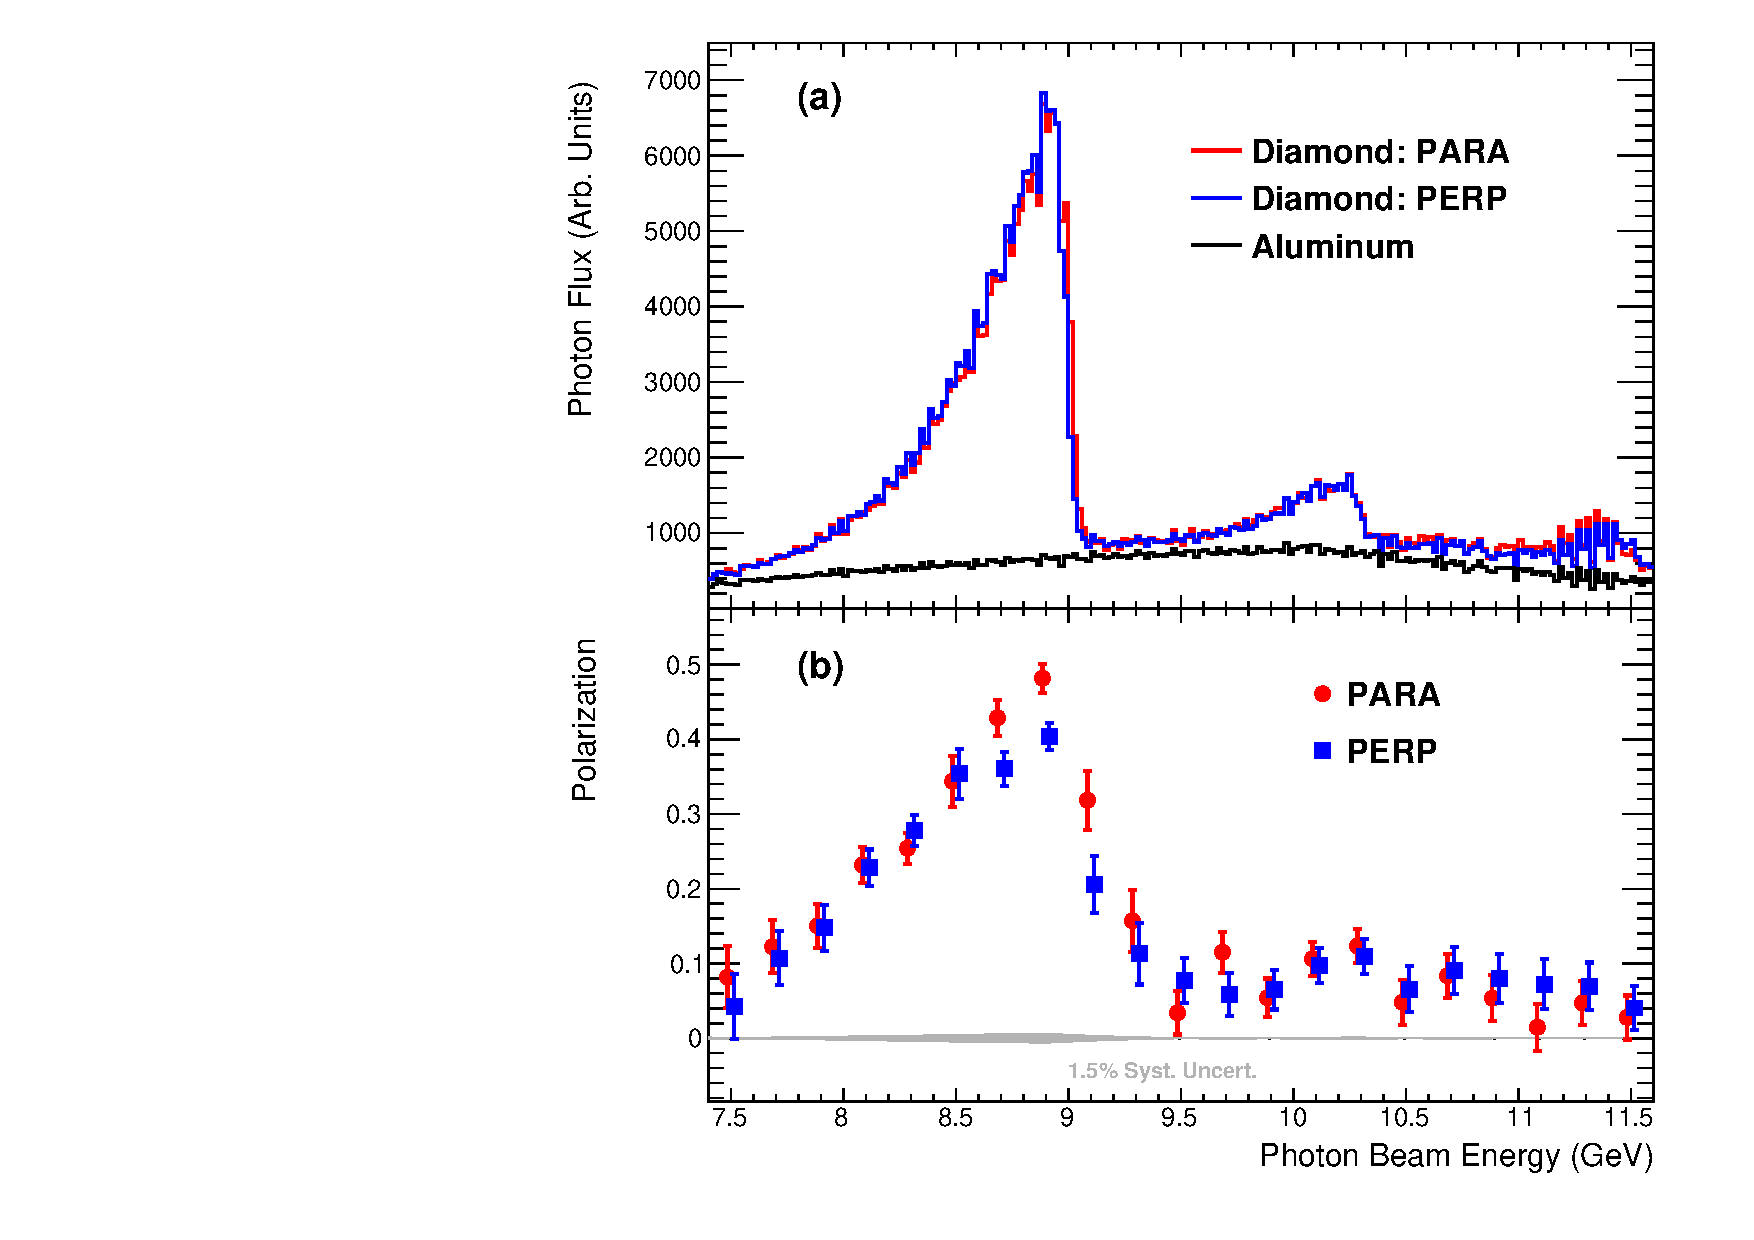
\includegraphics[clip=true,width=0.5\linewidth]{figures/gx3102_pi0etaAsym2016_fig0_beam.pdf}
\end{center}
\caption{(color online) (a) Photon beam intensity versus energy as measured by the pair spectrometer (not corrected for instrumental acceptance).  (b) Photon beam polarization as a function of beam energy, as measured by the triplet polarimeter, with data points offset horizontally by $\pm0.015$~GeV for clarity.
        }
\label{fig:beam:gx3102_pi0etaAsym2016_fig0_beam} 
\end{figure}



Finally, the photon beam travels through the \GX{} detector, and
ultimately goes to the photon beam dump just outside the downstream
end of the experimental hall.
The main parameters and properties of the Photon Beam are given in
Tables~\ref{tab:elecprop} and \ref{tab:operates}.




\begin{table}[tbp]
\begin{center}
\caption
[Assumed and projected electron beam properties]
{Electron beam parameters. The emittance, energy spread and
the related parameters were
predicted by a model of the transport line from
the accelerator to the Hall D photon source. }
\label{tab:elecprop}
\begin{tabular}{|l|c|}
\hline\hline
parameter & design results \\
\hline
extraction at & 5.5 passes \\
energy & 12~GeV \\
%electron polarization & available \\
energy spread, RMS & $<10$~MeV \\
transverse $x$ emittance & 10~mm$\cdot\mu$rad \\
transverse $y$ emittance & 2.5~mm$\cdot\mu$rad \\
$x$ spot size at radiator, RMS & 1.1~mm \ \\
$y$ spot size at radiator, RMS & 0.7~mm \ \\
$x$ image size at collimator, RMS & 0.5~mm \\
$y$ image size at collimator, RMS & 0.5~mm \\
distance radiator to collimator & 75.3~m \\
image position stability at collimator & $\pm$200~$\mu$m \\
\hline\hline
\end{tabular}
\end{center}
\end{table}


\begin{table}[tbp]
\begin{center}
\caption[Operating parameters for an experiment]{\label{tab:operates}
Operating parameters for an experiment using the coherent bremsstrahlung beam,
calculated with the properties
listed in Table \ref{tab:elecprop}, a diamond radiator of thickness 20 $\mu$m, and the standard
primary collimator of diameter 3.4~mm located at its nominal position.
The electron beam current is taken to 
be $2.2~\mu$A. The hadronic rates are calculated for 
a 30~cm liquid hydrogen target.}
%\begin{tabular}{|l|c|c|c|c|}
%\hline\hline
%$E$ upper edge of the peak & 8~GeV & 9~GeV & 10~GeV & 11~GeV \\
%Peak FWHM & 1140~MeV & 900~MeV & 600~MeV & 240~MeV \\
%$N_{\gamma}$ in the peak & 185~MHz & 100~MHz & 45~MHz & 15~MHz \\
%polarization in the peak & 0.54 & 0.41 & 0.27 & 0.11 \\
%%\multicolumn{1}{c}{(F.W.H.M.)} & (1140 \Meunit) & (900 \Meunit) & (600 \Meunit) & (240 \Meunit) \\
%%(F.W.H.M.) & (1140) & (900 \Meunit) & (600 \Meunit) & (240 \Meunit) \\
%peak tagging efficiency & 0.55 & 0.50 & 0.45 & 0.29 \\
%%\multicolumn{1}{c}{(F.W.H.M.)} & (720 \Meunit) & (600 \Meunit) & (420 \Meunit) & (300 \Meunit) \\
%(F.W.H.M.) & (720 \Meunit) & (600 \Meunit) & (420 \Meunit) & (300 \Meunit) \\
%power on collimator & 5.3 W & 4.7 W & 4.2 W & 3.8 W \\
%power on target & 810 mW & 690 mW & 600 mW & 540 mW \\
%total hadronic rate & 385 kHz & 365 kHz & 350 kHz & 345 kHz \\
%tagged hadronic rate & 26 kHz & 14 kHz & 6.3 kHz & 2.1 kHz \\

\begin{tabular}{|l|r|}
\hline\hline
$E$ upper edge of the peak & 9~GeV \\
Peak effective range       & 8.4 - 9.0~GeV\\
Tagger rate in the effective range & 240~MHz  \\
$N_{\gamma}$ in the effective range after collimator & 100~MHz  \\
Maximum polarization in the peak, after collimator & 41\% \\
Mean polarization in the effective range, after collimator & 37\% \\
Power on collimator & 4.5~W \\
Power on target & 0.7~W \\
Total hadronic rate & 360 kHz \\
Hadronic rate in the effective range & 15 kHz \\
\hline\hline
\end{tabular}
\end{center}
\end{table}


\subsection{Goniometer and Radiators \label{sec:radiators}}
The goniometer is a device which can position and precisely move horizontally, vertically and rotationally about the x, y and z axes.
The Hall D goniometer holds several radiators, each used depending on the requirements of the experiment.

For the linearly polarized photon beams typically used in \GX{} production running, diamond radiators are used in the coherent bremsstrahlung technique.
The properties of diamond make it suitable for use as the radiator in coherent bremsstrahlung; its small lattice constant and high Debye temperature result in small thermal motion of the atoms in the lattice, and its lattice structure suffers minimal thermal effects.

An important consideration when choosing a radiator is its thickness. The thickness of the radiator affects the angular divergence of the resulting photon beam, due to multiple scattering effects of the electron beam, and crystal defects in the radiator.
Minimising this divergence enhances the coherent bremsstrahlung spectrum, so the diamond used should be as thin as the considerations of manufacturing and
positioning of the radiator allow.
Hall D diamonds are typically 50-70 $\mu m$ thick.

%Coherent bremsstrahlung requires precise alignment of a diamond radiator, in order to produce a highly polarised beam by scattering off the appropriate crystal planes associated with a particular reciprocal lattice vector.


Several thin aluminium radiators, of varying thickness, are also available for collecting data to normalise the incoherent bremsstrahlung component from the linearly polarized beam data.

\begin{figure}[ht]
\begin{center}
   \includegraphics[page=4,viewport=581 1311 3020 2340,clip,angle=0,width=0.98\linewidth]{figures/D000000000-4002_RevB}
\end{center}
\caption{Tagger Hall layout
         from D000000000-4002
        }
\label{fig:beam:tagger-hall} 
\end{figure}

\subsection{Photon Tagging System \label{sec:tag}}
After passing through a radiator, the mixed photon-electron beam produced enters the photon tagging system (``tagger''), where the electrons are swept out of the beamline by a dipole magnet and detected by one of two systems in the tagger focal plane; the broadband hodoscope (TAGH) or the high resolution microscope (TAGM).
See Fig.\,\ref{fig:beam:tagger-hall}.
A permanent, 0.8~T$\cdot$m dipole magnet is located
downstream of the tagger magnet on the photon beam line, preventing
the electron beam to reach Hall D in case the tagger magnet trips.

Both the TAGM and TAGH devices are used to determine the photon beam energy via the relation $E_{\gamma} = E_{0} - E_{e}$, where $E_{0}$ is the primary electron beam energy from CEBAF, before interaction with the radiator, and $E_{e}$ is the energy of the electron determined by its detected position in the focal plane.
Electrons that did not interact with the radiator are swept into the electron beam dump.


\subsubsection{Tagger Magnet \label{sec:tagMagnet}}
The Hall D tagger magnet deflects electrons in the horizontal plane, allowing the bremsstrahlung-produced photons to continue to the experimental hall while having the electrons that produced them deposited in the focal plane detectors.
Electrons that lost a small amount of energy to bremsstrahlung in the
radiator, or did not interact with the radiator, are deflected by 13.4$^\circ$ into the electron beam dump.
Electrons that lost more than 25\% of their initial energy are deflected into the focal plane of the magnet, and are detected in either the TAGM or TAGH.

The Hall D tagger magnet is a dipole magnet 1.13 m wide, 1.41 m high and 6.3 m long, weighing 80 metric tons.
It has a normal operating field of 1.5 Tesla, with a maximum field of 1.75 T, and a pole gap of 30 mm


\subsubsection{Tagger Microscope (TAGM)}\label{sec:TAGM}
The Tagger Microscope is a high-resolution hodoscope that counts post-bremsstrahlung electrons corresponding to the photon energy band of interest to the experiment in Hall D.
For a 12 GeV incident electron beam, the microscope is used to tag photons between 8.4 and 9.0 GeV.
This energy changes depending on the primary electron beam energy, and the device is also designed to be movable to center on other energy ranges as demanded by experiment.

Scintillating fibre bundles are oriented towards the incoming electron axis in the tagger focal plane, and read out by silicon photomultipliers at the other end.
This detector provides fine segmentation along the direction of electrons' spread, increasing the energy resolution, as well as allowing selective readout to match the photon collimator acceptance through segmentation in the y-direction.

\subsubsection{Broadband Tagging Hodoscope (TAGH)}\label{sec:TAGHIntro}
The Tagger Hodoscope is a device consisting of $\sim$220 scintillator counters distributed over a length of 9.25 m and mounted just behind the focal plane of the tagger magnet.
Its function is to provide coarse sampling of the full photon energy range from 25\% to 97\% of incident electron energy (3.0 GeV to 11.7 GeV at an electron beam energy of 12 GeV).
This capability can be used to aid in alignment of the diamond radiator, as well as expand the \GX{} physics program to encompass photon energies other than the 9 GeV of the established program.
The gap in the coverage of the hodoscope scintillators is filled by the higher-resolution tagger microscope.

The construction of the hodoscope allows for later addition of counters to fully cover the energy range above the coherent peak for other microscope positions by filling the gaps between sampling scintillators. The mounting frame of the hodoscope is suspended from the Tagger-Hall ceiling to provide full flexibility of microscope positioning.

\subsection{Beam profiler}
The beam profiler is located in front of the collimator and is used to measure photon beam profiles.
The profiler consists of two planes of scintillator fibres, giving information on the photon beam profile in the X and Y directions.
Each plane is made up of 64 fibres, 2 mm in width, read out by eight multi-anode PMTs.

\subsection{Active collimator \label{sec:coll}}
The Active Collimator monitors the photon beam position and provides fast feedback to micro-steering magnets in the electron beamline, for the purpose of suppressing drifts in beam position.
It is located in the collimator cave area, on the front face of the primary collimator, and consists of a large tungsten plate, divided into two radial rings and four quadrants.

When a beam photon interacts with the plates, it creates a particle shower, detected by arrays of tungsten wires mounted parallel to the beam direction on each section of the Active Collimator.
These induce currents in the plate which indicate the degree of displacement of the beam from its intended center position.

\subsection{Collimator}
The photon beam produced at the diamond radiator contains both incoherent and coherent bremsstrahlung components.
In the region of the coherent peak, where photon polarization is at its maximum, the angular spread of coherent bremsstrahlung photons is less than that of incoherent bremsstrahlung.
The coherent radiation is concentrated at small angles $<$25~$\mu$rad with respect to the beam direction, while the incoherent radiation has a broader angular distribution.
To maximise the degree of linear polarization in the photon beam, it is tightly collimated.

The Hall D collimator provides apertures of 3.4 mm and 5.0 mm in a tungsten plate mounted on an X-Y table.
The entire collimator is surrounded by lead shielding.
In normal \GX{} running conditions, the 3.4 mm collimator is used.
The device also acts as the beam blocker, preventing high current beam, occasionally delivered by CEBAF for the purposes of beam tuning, from entering the experimental hall.
Several sweeping magnets are located along the collimator cave section of the beamline to remove unwanted charged particles from the photon beam.

\subsection{Triplet polarimeter \label{sec:tpol}}
The triplet polarimeter, or TPol, is used to measure the degree of polarization of the linearly polarized photon beam \cite{DUGGER2017115}.
The polarimeter uses the process of pair production on atomic electrons in a beryllium target foil, with these scattered atomic electrons measured using a silicon strip detector.
Information of the degree of polarization of the photon beam can be obtained by analysing the azimuthal distribution of the scattered atomic electrons measured by this device.

\subsection{Pair spectrometer \label{sec:ps}}

The Pair Spectrometer \cite{BARBOSA2015376} is located at the entrance to Hall D.
%(Fig.~\ref{fig:beam:hall-d}).
The spectrometer reconstructs the
energy of a beam photon by detecting the $e^\pm$ pair produced by the
photon in a thin converter. 
Electrons and positrons are registered in two layers of scintillator
detectors: a high-granularity hodoscope and a set of coarse counters,
referred to as PS and PSC, respectively.

The main purpose of the spectrometer is to measure the spectrum of the
collimated photon beam and determine the fraction of linearly polarized
photons in the coherent peak energy region.
It is also used to monitor the photon beam flux and can be used for 
energy calibration of the tagging hodoscope and microscope detectors.

%\subsubsection[Spectrometer]{Spectrometer\label{sec:beamline:ps-spetrometer}}

%Layout of the Hall D pair spectrometer is presented in Fig.~\ref{fig:beam:ps-layout}. 
% --------------------------------------------
%\begin{figure}[h]
%\begin{center}
%%   \tikzstyle{background grid}=[draw, black!50,step=.5cm]
%%   \begin{tikzpicture}[show background grid]
%%%   \begin{tikzpicture}[]
%%                  % The above right option is used to place the lower left corner
%%                  % of the image at the (0,0) coordinate. 
%%     \node [inner sep=0pt,above right] 
%%      {\includegraphics[angle=0,width=0.98\linewidth]{figs/ps_layout}};
%%       \node (halla)    at (2.0,0.3) [] {{\color{yellow} \scalebox{1.0}{\large A}}};  
%%       \draw[->,yellow,very thick] (halla) edge [] (3.25,1.75);
%%   \end{tikzpicture}
%   \includegraphics[angle=0,width=0.98\linewidth]{figs/ps_layout}
%\end{center}
%\caption{Pair Spectrometer simplified layout. In reality the detectors 
%         are tilted by 4.7$^\circ$ - perpendicular to the average trajectories.}
%\label{fig:beam:ps-layout} 
%\end{figure}
% --------------------------------------------

%Electron-positron pairs are created by beam photons inside a thin
%converter with a typical thickness ranging between 0.03\% and 0.5\% of
%a radiation length. The choice of the converter thickness depends on
%the photon beam flux. The maximum photon flux for GlueX physics runs
%is expected to be 50~MHz in the coherent peak energy region. Three
%converters with different thicknesses are installed in a movable fork
%that can insert one of them into the photon beam. Produced leptons are
%deflected in a 18D36 dipole magnet with an effective field length of
%about 0.94~m. The magnet was brought from Brookhaven National
%Laboratory and was modified at Jefferson Lab by reducing the pole gap
%from 6 inches to 3 inches. The magnet is operated at a nominal field
%of 1.8~T; the field integral is $\int{}Bdl\approx$1.60~T\,m. The beam
%angular spread is $<0.04$~mrad, and the angular spread of the pair
%production is $\sim{}\gamma^{-1}<0.2$~mrad. The multiple scattering at
%3~GeV in the thickest converter adds about 0.3~mrad. The particle
%deflection by the magnet at the momentum $p$ is
%$\theta{}=0.3\,[\mathrm{GeV/c/T/m}]\int{}Bdl/p$;
%$\theta\approx{}80~\mathrm{mrad}=4.6^\circ$ at 6~GeV.  
%A 1.5~m long vacuum chamber is installed after the magnet.
%Electrons and positrons are registered in two layers of scintillator detectors: a
%high-granularity hodoscope and a set of coarse counters, referred to as PS and PSC, respectively.
%The detectors are organized into two arms positioned symmetrically with
%respect to the photon beam line.  Each detector arm covers a momentum
%range of $e^\pm$ between 3.0 GeV/c and 6.2 GeV/c, corresponding to
%reconstructed photon energies between 6~GeV and 12.4~GeV. Relatively
%large acceptance of the hodoscope allows one to reconstruct photons
%with energies in the coherent peak energy region and also in the range
%near the beam end-point energy of 12~GeV. This can be used for the
%energy calibration of the hodoscope detectors.

%\begin{table}[h]
%  \begin{center}
%    \caption{The coordinates of the inner counters (the edge closest to the beam)
%             with respect to the magnet center. The survey was done at 2-Nov-2015. 
%       \label{tab:beam:ps-ccordinates}
%    }
%    %\vspace{3mm}
%    \begin{tabular}{l|r|r}
%       \hline
%       Detector & $Z$, mm & $X$, mm \\
%       \hline
%       \hline
%       PS~ Right arm & 2928.4 & -238.7 \\
%       PS~ Left~ arm & 2928.3 &  238.3 \\
%       PSC Right arm & 3416.2 & -274.4 \\
%       PSC Left~ arm & 3416.1 & ~274.8 \\
%       \hline
%    \end{tabular}
%  \end{center}
%\end{table}

%\subsubsection[PS: High Resolution Detector]{PS: High Resolution Detector
%  \label{sec:beamline:ps-hresol}
%}
%
%Each arm of the high resolution detector consists of 145 rectangular
%tiles made of EJ-212 scintillator~\footnote{
%  ELJEN Technology Plastic Scintillators \url{http://www.eljentechnology.com}. 
%}, stacked together as
%shown in Fig.~\ref{fig:beam:ps-tiles}. The tile height is 3 cm and the
%length along the particle path in scintillator is 1 cm. Out of 145 tiles,
%40 tiles close to the beam are 1~mm thick, the rest are 2~mm thick.
% The momentum bin size of the tile depends on the electron/positron energy as 
%%$\Delta{}p=\Delta{}x/x\cdot{}p$ 
%and constitutes about 13~MeV/c for 3~GeV and 24~MeV/c for 6~GeV particles.
%Tiles are optically isolated using 10~$\mu$m
%aluminized Mylar foil. This reflective foil also covers the bottom of
%the tile assembly. In order to keep the tiles parallel to the
%particle trajectories, the tiles are organized into 18 groups. Each
%group is tilted by $\sim$0.005~mrad using 0.05~mm thick shims
%(adhesive strips) positioned between the adjacent groups. The 
%first group is tilted by about 80~mrad, so that the tiles are parallel
%the 6~GeV particle trajectories.
%
%Light from a tile is collected using two 20~cm long 2$\times$2~mm$^2$
%double-clad BCF-92 wave-length shifting (WLS) fibers,
%glued to the sides of the tile using BC 600 Optical Cement. A tile
%assembly with two WLS optical fibers is shown in
%Fig.~\ref{fig:beam:ps-tiles}. The peak of the emission spectrum for EJ-212
%%scintillator occurs at the wavelength of 423 nm, which couples well
%with the absorption spectrum of the BCF-92 fiber. Light is
%subsequently re-emitted inside the fiber in the green range with an
%emission peak of 492 nm.
%
%Collected light is transmitted to the end of the WLS fiber. A pair of
%fibers from each tile is inserted into a hole in an aluminum mounting
%plate. %, as shown on the upper plot of Fig.~\ref{fig:hodoscope}. 
%The light detection is performed using Hamamatsu
%surface mount S10931-050P silicon photomultipliers with an effective
%photosensitive area of 3$\times$3~mm$^2$ and a pixel size of 0.05$\times$0.05~mm$^2$.
%These sensors have a photon detection efficiency (PDE) larger
%than 20\% at a wavelength of 500~nm and a typical gain of about
%$7\cdot{}10^5$~\footnote{
% Hamamatsu Corporation, MPPC S10931-050P, 
% \url{http://www.electronicsdatasheets.com/pdf-datasheets/hamamatsu/s10931050p}.
%}.
%Each photo sensor is coupled to two WLS fibers
%from a single tile.
%The electronics board (Fig.~\ref{fig:beam:ps-electr-assemb} left) 
%with 145 SiPMs is attached
%to the mounting plate.
%The SiPMs are arranged in two arrays
%of 3$\times$35 and 5$\times$8 sensors, which are connected to 2~mm and~1 mm
%tiles, respectively. SiPMs are optically isolated using a plastic
%spacer.
%
%
%% --------------------------------------------
%\begin{figure}[h]
%\begin{center}
%   \includegraphics[angle=0,width=0.45\linewidth]{figs/ps_tiles_photo_small}\hspace{0.05\linewidth}%
%   \includegraphics[angle=0,width=0.38\linewidth]{figs/ps_assembly_photo}
%\end{center}
%\caption{Scintillator tiles with two WLS fibers glued to sides of each tile: %30$\times$10$\times$1~mm$^3$ tile (left) 
%         and 30$\times$10$\times$2~mm$^3$  tile (right).
%        }
%\label{fig:beam:ps-tiles} 
%\end{figure}
%% --------------------------------------------
%
%% --------------------------------------------
%\begin{figure}[h]
%\begin{center}
%   \includegraphics[angle=0,width=0.43\linewidth]{figs/ps_sipm_plate_photo}\hspace{0.05\linewidth}%
%   \includegraphics[angle=0,width=0.47\linewidth]{figs/ps_assembly_drawing}
%\end{center}
%\caption{Electronics board with 145 SiPMs (left); 
%         the PS detector assembly (right).
%        }
%\label{fig:beam:ps-electr-assemb} 
%\end{figure}
%% --------------------------------------------

%\subsubsection[PSC: Coarse Resolution Detector]{PSC: Coarse Resolution Detector
%  \label{sec:beamline:ps-coarse} }
%
%Sixteen coarse scintillator counters, eight in each detector arm, are
%positioned about 40~cm behind the hodoscope.  The counters are 4.4~cm
%wide in the direction perpendicular to the particle trajectory, 2~cm
%thick, and 6~cm in height.  Hamamatsu R6427-01 PMTs are used to detect
%the scintillation light. The counters are used to produce a pair
%spectrometer trigger by requiring a coincidence of hits in the two
%detector arms. They also help to reduce background originating from
%interactions of $e^\pm$ inside the magnet pole edges to the level
%below 1\% by constraining the $e^\pm$ trajectories.  Counter rates
%depend on the converter thickness and photon beam flux. The maximum
%rate will not exceed 10~kHz per PSC counter during GlueX operation.
%
%
%\subsubsection[Electronics]{Electronics\label{sec:beamline:ps-electronics}}
%
%The PS hodoscope front end electronics consists of an amplifier and a
%SiPM bias voltage control circuit developed at Jefferson Lab. Signals
%from the SiPMs are amplified using the amplifier with a gain of about
%a factor of 20.  The amplifier is based on commercially available
%devices (operational amplifiers) with 3~GHz bandwidth.  Pulse shaping
%is employed to compensate for the characteristically high SiPM
%capacitance and package inductance. The impulse response shows rise
%and fall times of 3~ns and with trans-impedance gain of 1~mV/$\mu$A.  
%The SiPM operating bias voltage is about 73~V. The
%nominal bias setting is as specified by Hamamatsu (1~V over voltage)
%and fed to the SiPM through a resistive network employing a thermistor
%and a linearizing resistor. The hodoscope control electronics supply
%individually adjusted voltages to groups of 5 SiPM channels; inside
%the group the voltage is adjusted among channels using resistors. The
%thermistor senses the average temperature of closely packed SiPMs in
%thermal equilibrium via a heat spreader PCB layout, thus forming a
%well controlled loop. 
%%The commercially available bias power supply has
%%very low noise characteristics and is well regulated to less than 1~mV
%%long term. The supply allows the user to monitor and adjust the levels
%%as needed and if required. The optimal bias setting will be determined
%%based on experimental conditions.
%
%Signals from both the hodoscope and coarse counters are digitized
%using a twelve-bit multi-channel flash ADC operated at a sampling rate
%of 250~MHz (fADC250-MHz). The PSC counters are also instrumented with
%TDCs, with the intrinsic resolution of $\sim$60~ps.  The timing resolution
%is expected to be better than 200~ps. 
%
%An example of the fADC signal pulse obtained from a PS scintillator
%tile is shown in Fig.~\ref{fig:beam:ps-signals} (left).  The ADC
%sampling time is 4~ns. The SiPMs allow to resolve the number of pixels
%fired, demonstrated in Fig.~\ref{fig:beam:ps-signals} (right). The
%average amplitudes of the signals in the Pair Spectrometer correspond
%to about 60 pixels fired.
%
%%This resolution will allow one
%%to distinguish the electron beam bunch where the bremsstrahlung photon
%%is emitted and therefore relate hits from the pair spectrometer and
%%tagging detectors originating from the same event.
%
%% --------------------------------------------
%\begin{figure}[h]
%\begin{center}
%   \includegraphics[angle=0,width=0.45\linewidth]{figs/ps_sipm_pulse}\hspace{0.05\linewidth}%
%   \includegraphics[angle=0,width=0.45\linewidth]{figs/ps_sipm_pixels_peaks}
%\end{center}
%\caption{PS typical fADC250-MHz signal (left); 
%         PS The spectrum of fADC signals integrated in 60~ns, obtained using a low intensity light source. 
%         The spectrum
%         resolves the peaks from different numbers of pixels fired,
%         including zero (the pedestal) (right).
%        }
%\label{fig:beam:ps-signals} 
%\end{figure}


\subsection{Total absorption counter \label{sec:tac}}
The Total Absorption Counter (TAC) is a high-efficiency lead glass calorimeter, used at low beam currents ($<5$nA) to determine the overall efficiency of the coherent bremsstrahlung facility.
Not every photon produced at the radiator reaches the hall, and in normal \GX{} running not every photon that reaches the hall causes an interaction detected in the \GX{} detector.

Using the TAC at normal \GX{} production currents is not possible, as it would very quickly succumb to radiation damage, therefore the TAC is used to measure photons reaching it at low currents with near 100\% efficiency.
From this measurement, the fraction of bremsstrahlung produced photons reaching \GX{} at nominal operational beam currents can be determined by extrapolation.

\subsection{Flux normalization \label{sec:fluxnorm}}
(Status 09/30/2019: Materials collated, section will be included after collaboration meeting)

\subsection{Photon polarization (M. Dugger/ASU Student)\label{sec:polarization}}